\documentclass[a4paper, 11pt, twocolumn]{article}

%Handige usepackages voor essays
%\usepackage[protrusion=true,expansion=true]{microtype} % Better typography
%\usepackage{graphicx} % Required for including pictures
%\usepackage{wrapfig} % Allows in-line images
%\usepackage{mathpazo} % Use the Palatino font
%\usepackage[T1]{fontenc} % Required for accented characters
%\linespread{1.05} % Change line spacing here, Palatino benefits from a slight increase by default

%Handige usepackages voor essays
%\usepackage[protrusion=true,expansion=true]{microtype}
%\usepackage{microtype}
\usepackage{graphicx} % Required for including pictures
\usepackage{wrapfig} % Allows in-line images
%\usepackage{mathpazo} % Use the Palatino font
%\usepackage[T1]{fontenc} % Required for accented characters
%\linespread{1.05} % Change line spacing here, Palatino benefits from a slight increase by default

%Standaard usepackages
\usepackage{pdfsync}
\usepackage[english]{babel}
\usepackage{fullpage}
\usepackage{amsmath}
\usepackage[table]{xcolor}
\usepackage{caption}
\usepackage{subcaption}
\usepackage{float}
\usepackage{verbatim}
\usepackage{eso-pic}
\usepackage[toc,page]{appendix}
\usepackage[linkbordercolor={white}]{hyperref}
\usepackage{nameref}
\usepackage{listings}
\usepackage{filehook}
\AtEndOfIncludes{%
  \global\let\savedclearpage\clearpage
  \global\let\clearpage\relax
}
\AfterIncludes{%
  \global\let\clearpage\savedclearpage
}
\makeatletter
\renewcommand{\@listI}{\itemsep=0pt} % Reduce the space between items in the itemize and enumerate environments and the bibliography

\renewcommand{\maketitle}{ % Customize the title - do not edit title and author name here, see the TITLE block below
\begin{flushright} % Right align
{\LARGE\@title} % Increase the font size of the title

\vspace{50pt} % Some vertical space between the title and author name

{\large\@author} % Author name 1
\\\@date % Date

\vspace{40pt} % Some vertical space between the author block and abstract
\end{flushright}
}

%----------------------------------------------------------------------------------------
%	TITLE
%----------------------------------------------------------------------------------------

\title{\textbf{Hardware Implementations of Evolvable Systems}\\ % Title
A critical analysis on self-adaptive autonomic systems on reconfigurable architectures } % Subtitle

\author{\textsc{Imara Speek \\ 
Aimee Ferouge} % Author
\\{\textit{Delft University of Technology}}} % Institution

\date{\today} % Date

%----------------------------------------------------------------------------------------

\begin{document}

\twocolumn[
	\begin{@twocolumnfalse}
	\maketitle
	\begin{abstract}
	%----------------------------------------------------------------------------------------
	%	ABSTRACT AND KEYWORDS
	%----------------------------------------------------------------------------------------

	%\renewcommand{\abstractname}{Summary} % Uncomment to change the name of the abstract to something else

	Morbi tempor congue porta. Proin semper, leo vitae faucibus dictum, metus mauris lacinia lorem, ac congue leo felis 	eu turpis. Sed nec nunc pellentesque, gravida eros a. 
	lobortis ultrices eget ac metus. In tempus hendrerit rhoncus. Mauris dignissim turpis id sollicitudin lacinia. Praesent 		libero tellus, fringilla nec ullamcorper at, ultrices i nulla. Phasellus placerat a tellus a malesuada.
	\end{abstract}

	\hspace*{3,6mm}\textit{Keywords:} bio-inspired , self-aware , computing systems, machine learning % Keywords
		
	\vspace{30pt} % Some vertical space between the abstract and first section
	\end{@twocolumnfalse}
]

%----------------------------------------------------------------------------------------
%	ESSAY BODY
%----------------------------------------------------------------------------------------
Blabla

% Introduction

\section*{Introduction}

*Introduction* \cite{fpga} blabla \cite{why}

%prior knowledge
\section{Fundamental knowledge}
\label{sec:fundamental}
In this section an introduction to the fundamental terms used in this paper is given. These terms concern prior knowledge required when working with autonomic or evolvable systems and their implementations in hardware. 

Computing system containing \emph{self-properties} are capable of adapting their behavior and resources thousands of times based on changing environmental conditions and demands \cite{selfaware}. This allows them to automatically accomplish their goals in the best way possible. This behavior is achieved through \emph{self-monitoring} which recognizes changes in its internal state that may require a modification, called \emph{self-adjusting}. \emph{Self-healing} concerns effective recovery under fault condition, \emph{self-optimization} invokes optimizing operation in proactive and reactive manners and \emph{self-configuring} concerns automatically installing, configuring and integrating new components seamlessly into the system to meet stated goals \cite{autocom}. 

%\subsection{Evolvable systems}
% what is evolvable
\emph{Evolvable systems} exploit self-adaptive, self-configuring and self-optimizing techniques and are capable of changing their operations to meet the given performance goals by modifying either the underlying heterogeneous architecture, the operating system and the self-adaptive applications. \cite{evolvable}
%Meeting efficiency and accuracy constraints is getting more and more difficult , mainly because of the exponential increase of interactions among systems and the environments in which the systems are required to work. 
%The operating systems chooses at run-time among a set of possible implementations according %to the criteria. This decision is based on the Observe-decide-act. The need for this dynamic %choice between available implementations is give by the fact that the system is live and %lives in an unpredictable environment. \cite{selfaware}

%e explanation of autonomic 
\emph{Autonomic systems} are inpired by the human body's nervous system and contains all self-properties: \emph{self-managing, self-protecting, self-healing} and \emph{self-optimizing} \cite{autonomic}. 

Autonomic and evolvable systems have the need for heterogeneous underlying architectures, which can be provided by using Field Programmable Gate Arrays (FPGAs).These can be configured to fullfil a desired functionality by using one or more bitstreams. These bitstreams are binary files in which FPGA specific configuration information is stored and these are to be copied along with the proper commands on to the configuration SRAM cells, or the configuration memory \cite{reconfigurable}. 
% Discussion of the papers

\section{Discussion of the Different Papers}
\label{sec:discussion}

\emph{[introduction to discussions and seperation of the topics, maybe seperate hardware from software solution from these papers?]
[Give some small introduction to each paper in 3 sentences and then maximum of 15 for every paper]}
\\
\\
Considerable research has already been done in order to efficiently accelerate hardware while still maintaining virtually unlimited adaptability. 
Software techniques in autonomic computing systems such as hot-swapping and data clustering are discussed in \cite{survey}. 
These self-aware systems can adapt their behavior on FPGA-based system as discussed in \cite{selfaware}.
Other approaches start with a FPGA-based architecture with a reconfigurable core \cite{drp},  added programming schemes and new cell structures \cite{virtex4}, \cite{erlangen} or even bio-inspired hardware using the POE-model \cite{poe}.
More recent papers put effort a combined approach by either implementing autonomic systems on reconfigurable architectures \cite{reconfigurable} or creating evolvable systems via self-aware applications \cite{evolvable}.

%% -- Software based papers --------------------------
\subsection{Software based flexible approaches}
\label{sec:software}

%%Survey of Frameworks, Architectures and Techniques in Autonomic Computing

Self-configuration is the ability of the system to perform configurations according to the pre-defined high level policies and seamlessly adapt to change caused by automatic configurations. Self-optimization is the ability of the system to continuously monitor and control resources to improve performance and efficiency. Self-healing is the ability of the system to automatically detect, diagnose and repair faults. Self-protection is the ability of the system to pro-actively identify and protect itself from malicious attacks or cascading failures that are not corrected by self-healing measures.

This paper presents a wide variety of techniques in autonomic computing. Hot-swapping is a technique to inject monitoring and diagnostic code into live code using inter-positioning and replacement. Data clustering is an unsupervised learning algorithm, used to identify configuration classes and determines the degree of similarity between clusters using convex average metric.

				% April, 2009, maybe use this only for prior knowledge
% Software based approaches
The \emph{Heartbeats application} is a monitoring application which makes it possible to assert performance goals as heart-rate windows delimited by a minimum and maximum performance, or \emph{heart-rate} \cite{evolvable}. The Heartbeats API is made of small straightforward functions and allows declaring performance goals. Software components first have to register, specifying parameters such as minimum and maxmim heart-reate, size of the windows of observation and history buffers \cite{selfaware}. The application then updates the progress of the execution calling the function that signifies a heartbeat \cite{evolvable}.

%[SMARTLOCKS PAPER] presents a combination of the Heartbeats application in cooperating with other frameworks. Smartlocks is a spinlock library that will adapt its internal implementations based on defined goals during run-time using heurstics as discussed in subsection \ref{sec:decisions} and machine learning. 

\cite{reconfigurable} dscusses using adaptive programming in situations where input changes lead to relatively small output changes. They present a hardwar/software codesign paradigm that develops a new performance model and associated evaluation metrics to differentiate between various levels of performance across different portions of software modules. Incoorporating this into a codesign environment increases the flexibility of the system. 
%distributed self trained algorithms, machine learning, heartbeats application
%adaptive programming

%% -- Hardware based papers --------------------------
\subsection{Hardware based fast approaches}
\label{sec:hardware}

%% A Phylogenetic, Ontogenetic, and Epigenetic View of Bio-Inspired Hardware Systems

As a final category of evolvable systems, inspired by life on Earth and the natural processes of living organisms, \emph{bio-inspired} hardware systems have evolved. \cite{poe} introduces the POE model, that classifies bio-inspired systems according to three axes:
\begin{itemize}
	\item Phylogeny, where evolvable hardware can be found.
	\item Ontogeny, where systems have the ability to self-repair as the main goal of ontogeny is (cell) growth or construction.
	\item Epigenesis, which is more software-based.
\end{itemize}

By looking at these biological phenomena, researchers can be inspired when developing evolvable hardware systems.					% August, 2002
% The Erlangen Slot Machine: A Dynamically Reconfigurable FPGA-based Computer
\label{sec:erlangen}
FPGAs are commonly used device for implementing the reconfigurable architecture of evolvable systems, especially Virtex FPGAs produced by Xilinx. The \emph{Erlangen Slot Machine (ESM)} from \cite{erlangen} tackles the three major limitations of the Virtex-II FPGA. A pipelined data flow architecture has been used, replacing the finite state machine by a MicroBlaze microcontroller and employing a data crossbar between plug-ins. The ESM has proven to be a valid alternative to the Virtex FPGAs, providing a new architecture to overcome current physical shortcomings of the reconfigurable FPGAs, as well as a new inter-module communication concept and an intelligent module reconfiguration management. 
			% April, 2007
% A Direct Bitstream Manipulation Approach for Virtex4-based Evolvable Systems

In \cite{virtex4} a Virtex4 FPGA implementation is introduced for evolvable systems. Other then earlier versions of Virtex (e.g. the Virtex-II Pro), Virtex4 devices enable two-dimensional dynamic reconfiguration, a feature which considerably reduces the reconfiguration time an thus the evoltuion time (\cite{virtex4}). By using both VRCs (Virtual Reconfigurable Circuits) and direct bitstream manipulation, this new architecture eliminates the biggest limitation of Virtex FPGAs, which is an almost unknown and undocumented bitstream data format and an unsafe configuration schema. 

This Virtex4-based device, which takes advantage of 2D reconfiguration capabilities and direct manipulation of the bitstreams is the first one of its kind and will be discussed later.				% May, 2010
% A Fast Reconfigurable 2D HW Core Archtiecture on FPGAs for Evolvable Self-Adaptive Systms

Another Virtex-4 based architecture introduced in \cite{dpr} also applies the 2D reconfiguration core. Rather than direct bitstream manipulation, a \emph{dynamically partial reconfiguration (DPR)} control engine has been integrated. As a result, the processing elements (PEs) of the reconfigurable core are structured as a 2D systolic array, known for its high performance and restrained use of resources. The reconfiguration engine has been optimized by applying three enhancements that will be discussed in \ref{sec:dpr}.					% June, 2011

%% -- Combinations based papers ----------------------
\subsection{Co-design based systems}
\label{sec:codesign}

% From reconfigurable architectures to self-adaptive autonomic systems 
\cite{reconfigurable} proposes the harvesting of the full potential of dynamic reconfiguration by carefull evaluating the overhead of reconfiguration in hardware-software interfacing. To overcome the limits introduced by increasing complexity and the workloads to main complex infrastructues they propose to adopt a codesigned self-adaptive and autonomic computing system. 
%A full \emph{bitstream} configures the whole configuration memory statically at the beginning of the execution of a system, while partial bitstreams are used for reconfiguration to confirgure merely portions of the device. 

\emph{Partial dynamic reconfiguration (PRD)} is a key feature that makes FPGAs unique. PDR addresses the lack of resources to implement an application and its adaptability needs. Reconfigurable hardware taking advantage of partial dynamic reconfiguration is the perfect trade-off between the speed of HW and the flexibility of SW. \cite{reconfigurable} present an evaluation system, implemented on the Xilinx Virtex-II Pro VP30 on an architecture of two reconfigurable cores. Running an extended version of Linux, the cores can be partial dynamically reconfigured. They compare the performance of three different impementations of a popular encryption algorithm (advanced encryption standard): a reconfigurable IP-core that is configured at runtime (FPGA-RHW), a cached hardware IP-core that is ready to use (FPGA-CHW) and a software implementation (SW) as can be seen in figure \ref{fig:reconfig}. 
% -- reconfig, cached & software ---------------------------
\begin{figure}[htb]%
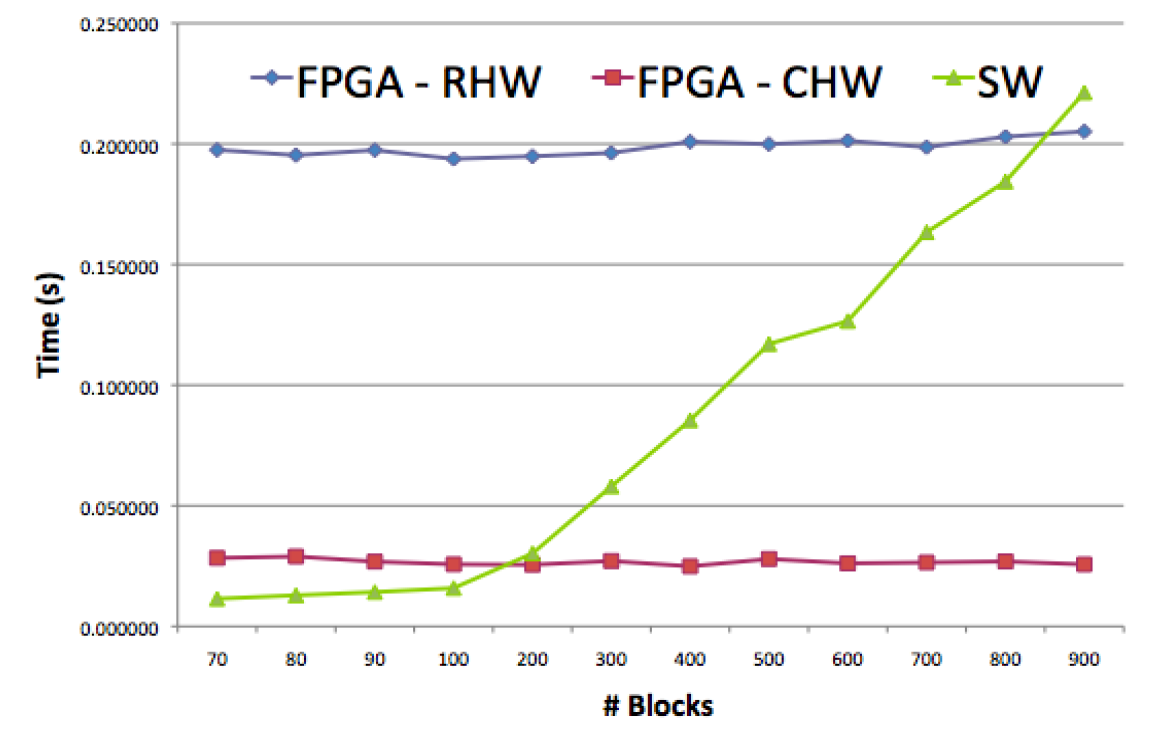
\includegraphics[width=\columnwidth]{Pictures/reconfig.png}%
\caption{Execution time of the implementations of the AES algorithm as seen in \cite{reconfigurable}}%
\label{fig:reconfig}%
\end{figure} 
Figure \ref{fig:reconfig} displays the overhead introduced by reconfiguration. Even though this data was captured in a static analysis, it displays that reconfiguration may dominate the execution. This shows the need for a efficient and fast decision engine, as reconfiguration seems to be only valid in systems of larger than 900 processed blocks. 
%
%However, an important problem often neglected is the time overhead the reconfiguration process introduces and the two-dimensional partitioning strategy reconfigurable devices need: spatial and temporal. \cite{reconfigurable} presents the urge to carefully evaluate the overhead created as a negative impact of reconfiguration latency which is not always discussed in present papers. 
% Evolvable systems on reconfigurable architecture via self-aware adaptive applications. ++
In \cite{evolvable} an evolvable system running self-adaptive application on top of a heterogeneous systems is proposed. 
The operating system running on top is responsible for providing the self-* proporties and runs this on a general purpose processor and a reconfigurable device 

In \cite{evolvable}, the underlying hardware architecture is made up of  static area and a dynamic area. The reconfigurable device can be configured to implement different functionality through dynamic reconfiguration support provided by the operating system. This is provided through standard libraries and the OS implements parts of the loop. The OS is therefor capable of choosing at run-time the best implementation for the required functionality among the available.
The switchable units in the hot-swap method in \cite{evolvable} are identified as the libraries that export an implementation of a certain functionality. 
The self-adaptive library or Dynamic-link library(DLL) and the software implementation library target the reconfigurable FPGA and multicore respectively. 


% Comparison of the papers

\section*{Comparison}

*Comparison*

% Proposition of a evolvable system on a reconfigurable architecture

\section{Proposed Adaptive System Design}
\label{sec:proposition}

Given all these techniques, the question rises which of them could become promising when being combined with each other. In this section, a design is being proposed mixing and matching the previous techiques based on their advantages and drawbacks. By doing this, we first look at the hardware implementations, since these are responsible for the physical limitations. Afterwards, several software techniques are considered in order to add the evolvable behaviour to the system.

% --- HW Proposal --------------------------------------

\subsection{Proposed Hardware}
\label{sec:hardware}

The architecture introduced in \cite{PDR} seems the most promising architecture. Whereas \cite{virtex4} is still discovering the two-dimensional reconfigurability using rigid columns with static routing, \cite{PDR} is applying \emph{Partial Dynamically Reconfiguration}, enabling the system to reconfigure certain parts while others keep running their program. Keeping the idea of evolvable systems in mind, this feature enables an \emph{autonomic system} best. Also, the designers have used their one drawback (the addition of an enhanced ICAP) to include two more system improvements concerning the speed up. 

A quantative comparison between all three the hardware implementations will be covered in Section \ref{sec:related}.

% --- SW Proposal --------------------------------------------
\subsection{Proposed Software}
\label{sec:prosoftware}
The evolvable framework co-designed with the proposed hardware has to include a monitoring technique, a decision making engine and an adaptation framwork. The Evolutionary Framework proposed in \cite{PDR} is based on an evolutionary algorithm that uses static input data files as reference for its evolution. This section proposed an adaptable fully autonomous system on top of our heterogeneous architecture. 

The \emph{HeartBeats application} is proposed as the monitoring technique as it enables the system to predefine performance goals and delivers real-time information to the decision engine. This will introduce a moderate overhead by initializing the data structures which will relatively decrease when dealing with larger complex systems. This is acceptable as Section \ref{sec:codesign} displayed that the use of evolvable system only becomes valid when working with these complex systems. This run-time information will support an agile self-aware system. 

The monitoring system will feed the performance information to the decision engine. Inspired by the PDR methods a partial dynamic model is proposed. A combination of an \emph{analytical} and \emph{empirical model} will enhance the initial performance of the system as it has priorly developed knowledge in the analytical model. The empirical model can take over when performance goes out-of -bounds to handle unexpected behavior. 

PDR will reduce the amount of overhead introduced by reconfiguration during self-adapting. However a framework to adapt, or switch between implementations of functionalities still has to be provided. The \emph{Implementation Switch Service} inspired by the \emph{hot-swap mechanism} as proposed in \cite{selfaware} solves the state quiescence and state translation and thus completes the proposed evolvable framework.


% Conclusion and Future Challenges

\section{Conclusion}
\label{sec:conclusion}
In this paper, a hardware implementation of an evolvable system is proposed. The two-dimensional reconfigurable architecture using systolic arrays of processing elements enabling partial dynamically reconfiguration and its co-designed evolvable framework supporting the HeartBeats monitoring application an empirical model based decision engine and a hot-swap inspired self-adapting framework is based on a critical analysis of current research in autonomic and evolvable systems on heterogeneous architectures. 

The proposed design was derived after discussing current research in the field of evolvable systems and heterogeneous architectures and extracting the techniques that are utilized. Although a deeper understanding is given into the world of autonomic systems, future work would have to invest in providing an analytical understanding. Proposed future work would be running benchmarks for these systems so the techniques that were used can be compared seperately and in co-design. 

This paper provides a deeper understanding into co-design of hardware and software that is becoming increasingly important considering the current increase in system complexity and size.

%----------------------------------------------------------------------------------------
%	BIBLIOGRAPHY
%----------------------------------------------------------------------------------------

\bibliographystyle{plain}

\bibliography{References}

%----------------------------------------------------------------------------------------

\end{document}